\section{Method}

\subsection{Problem Formulation}

Let $f_\theta$ be a promptable segmentation model that takes a 3D image $\mathbf{x} \in \mathbb{R}^{D \times H \times W}$ and a point prompt $p = (d, h, w)$ to produce a binary mask $f_\theta(\mathbf{x}, p) \in \{0,1\}^{D \times H \times W}$. We define \emph{prompt faithfulness} as the property that changing the prompt target changes the prediction accordingly.

\paragraph{Switch Accuracy.}
Given an image $\mathbf{x}$ containing organs $A$ and $B$ with ground-truth masks $y_A$ and $y_B$, and prompts $p_A \in A$, $p_B \in B$, we define a \emph{switch} as successful if both conditions hold simultaneously:
\begin{equation}
\text{Dice}(f_\theta(\mathbf{x}, p_A), y_A) > \text{Dice}(f_\theta(\mathbf{x}, p_A), y_B)
\label{eq:switch1}
\end{equation}
\begin{equation}
\text{Dice}(f_\theta(\mathbf{x}, p_B), y_B) > \text{Dice}(f_\theta(\mathbf{x}, p_B), y_A)
\label{eq:switch2}
\end{equation}
Switch Accuracy is the fraction of paired prompts satisfying both conditions across a fixed evaluation bank. This metric captures whether the model produces the \emph{correct} organ for each prompt, not merely whether it produces \emph{something}.

\subsection{Why Standard Training Fails}

Standard training optimizes $\mathcal{L}_{\text{seg}}(f_\theta(\mathbf{x}, p), y)$ independently for each prompt. This objective is satisfiable without prompt faithfulness: a model that always predicts the largest organ achieves reasonable Dice regardless of prompt location. Formally, if organ $A$ dominates the volume, then $f_\theta(\mathbf{x}, p) \approx y_A$ for all $p$ achieves high average Dice without ever using $p$. The loss contains no term enforcing that $f_\theta(\mathbf{x}, p_A) \neq f_\theta(\mathbf{x}, p_B)$ when $A \neq B$.

This explains why standard LoRA fine-tuning (seg-only) improves Dice from 0.450 to 0.720 but Switch Accuracy only reaches 0.483---the model learns better segmentation but not better prompt following.

\subsection{Paired Prompt-Contrastive Training}

We address this by training with paired prompts (Figure~\ref{fig:framework}). For each image $\mathbf{x}$ containing organs $A$ and $B$:
\begin{enumerate}
    \item Compute image embedding $\mathbf{e} = \text{Enc}(\mathbf{x})$ once (frozen encoder)
    \item Decode with prompt $p_A$: $\hat{y}_A = \text{Dec}_\phi(\mathbf{e}, p_A)$
    \item Decode with prompt $p_B$: $\hat{y}_B = \text{Dec}_\phi(\mathbf{e}, p_B)$
    \item Supervise both predictions against respective ground truths
\end{enumerate}

The decoder $\text{Dec}_\phi$ (prompt encoder + mask decoder) is shared between both passes and adapted via LoRA~\citep{hu2022lora} with rank 8, yielding 1.9M trainable parameters (1.89\% of total 100.5M). The image encoder remains frozen, so the second forward pass reuses the cached embedding $\mathbf{e}$ with minimal overhead.

\begin{figure*}[t]
\centering
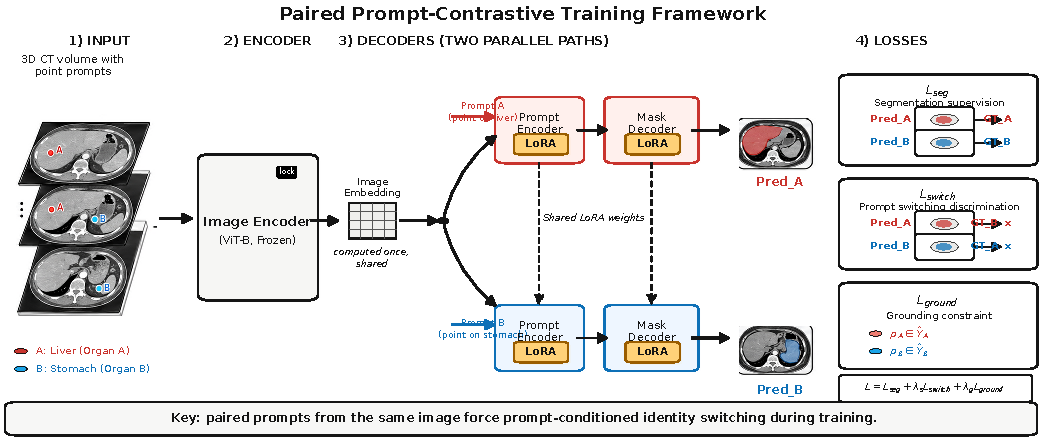
\includegraphics[width=0.95\textwidth]{figures/fig2_training_framework.pdf}
\caption{Paired Prompt-Contrastive Training framework. The frozen image encoder computes a shared embedding. Two different organ prompts are decoded through the same LoRA-adapted decoder, producing two predictions supervised by their respective ground truths. The switch margin loss enforces that each prediction is closer to its target organ than to the alternative.}
\label{fig:framework}
\end{figure*}

\paragraph{Loss Function.}
The total loss combines three terms:
\begin{equation}
\mathcal{L} = \mathcal{L}_{\text{seg}} + \lambda_s \mathcal{L}_{\text{switch}} + \lambda_g \mathcal{L}_{\text{ground}}
\label{eq:total_loss}
\end{equation}

The segmentation loss averages Dice+BCE on both predictions:
\begin{equation}
\mathcal{L}_{\text{seg}} = \frac{1}{2}\left[\ell(\hat{y}_A, y_A) + \ell(\hat{y}_B, y_B)\right]
\end{equation}

The switch margin loss enforces output separation:
\begin{multline}
\mathcal{L}_{\text{switch}} = \left[m + D(\hat{y}_A, y_B) - D(\hat{y}_A, y_A)\right]_+ \\
+ \left[m + D(\hat{y}_B, y_A) - D(\hat{y}_B, y_B)\right]_+
\label{eq:switch_loss}
\end{multline}
where $D(\cdot,\cdot)$ is soft Dice similarity, $m{=}0.2$ is the margin, and $[\cdot]_+ = \max(0, \cdot)$. This loss penalizes predictions that are more similar to the wrong organ than to the correct one, maintaining a persistent gradient signal throughout training.

The grounding loss ensures prompt points lie inside predictions:
\begin{equation}
\mathcal{L}_{\text{ground}} = -\log\sigma(\hat{y}_A[p_A]) - \log\sigma(\hat{y}_B[p_B])
\end{equation}
where $\sigma$ is the sigmoid function and $\hat{y}[p]$ denotes the logit at the prompt location.

We use $\lambda_s{=}1.0$ and $\lambda_g{=}0.5$ throughout. As our ablation demonstrates (\S\ref{sec:mechanism}), the specific loss weights matter far less than the paired training paradigm itself.

\paragraph{Key Insight.}
The critical mechanism is not any particular loss function but the \emph{paired prompt exposure}: by presenting two different prompts for the same image in a single training step, the model cannot satisfy the objective by ignoring prompts. It must learn to condition its output on the prompt to minimize loss on both predictions simultaneously.
